\documentclass[10pt,a4paper,twocolumn]{article}
\usepackage[T1]{fontenc}
\usepackage[utf8]{inputenc}
\usepackage{lmodern}
\usepackage[ngerman]{babel}
\usepackage[margin=2cm,columnsep=0.8cm]{geometry}
\usepackage{microtype}
\usepackage{graphicx}
\usepackage{booktabs}
\usepackage{caption}
\usepackage{subcaption}
\usepackage{xcolor}
\usepackage{listings}
\usepackage[round,authoryear]{natbib}
\usepackage[hidelinks]{hyperref}
\captionsetup{font=small,labelfont=bf}
\setlength{\parindent}{1em}
\graphicspath{{results/abbildungen/}}
\lstset{basicstyle=\ttfamily\footnotesize,breaklines=true,columns=fullflexible,
        frame=single,rulecolor=\color{black!25},showstringspaces=false}

% Rot markierte Stellen musst du noch selbst eintragen oder pruefen
\newcommand{\todo}[1]{\textcolor{red}{[#1]}}

\title{Verwandtschaftsanalyse aus öffentlichen Genomdaten: Mendel-Fehler und KING an vier Personen der CEPH-Familie 1463}
\author{Karim Andjar\\[2pt]\small Masterstudiengang Bioinformatik und Systembiologie, Justus-Liebig-Universität Gießen}
\date{}

\begin{document}
\twocolumn[
\maketitle
\begin{center}
\begin{minipage}{0.92\textwidth}
\small
\textbf{Zusammenfassung.}
Ich habe für vier Personen der CEPH-Familie 1463 (NA12877, NA12878, NA12891, NA12892) aus öffentlichen Ganzgenomdaten bestimmt, wer mit wem verwandt ist, ohne die Rollen vorzugeben. Dazu habe ich eine Snakemake-Pipeline aufgebaut: Mapping (BWA-MEM), Duplikatmarkierung (GATK), Variantenbestimmung (HaplotypeCaller im GVCF-Modus), gemeinsame Genotypisierung und Filterung auf SNPs der Chromosomen 20 bis 22 (329.422 SNPs). Ausgewertet wurde mit zwei unabhängigen Verfahren, der Zählung von Mendel-Fehlern und dem KING-robust-Schätzer. Beide ergeben dasselbe Bild: NA12878 ist das Kind von NA12891 und NA12892, und NA12877 ist mit keiner dieser Personen verwandt. Die Mendel-Fehlerrate liegt für die beiden Eltern-Kind-Paare bei 0,015~\% und 0,096~\%, für alle übrigen Paare bei 5,4 bis 5,9~\%, und das beste Trio (0,65~\%) liegt um etwa das 21-Fache unter der nächstbesten Kombination. Die absoluten KINSHIP-Werte sind in dieser kleinen Kohorte für alle Paare nach oben verschoben; belastbar sind IBS0 und die Rangfolge. Es wurden nur drei Chromosomen und vier Personen untersucht.

\medskip
\textbf{Abstract.}
For four members of the CEPH family 1463 (NA12877, NA12878, NA12891, NA12892), I inferred relatedness from public whole-genome data without assigning roles in advance. A Snakemake pipeline (BWA-MEM, GATK MarkDuplicates and HaplotypeCaller in GVCF mode, joint genotyping) produced 329,422 SNPs on chromosomes 20 to 22, which were analysed by counting Mendelian errors and with the KING-robust estimator. Both methods agree: NA12878 is the child of NA12891 and NA12892, and NA12877 is unrelated to all three. The Mendelian error rate is 0.015\% and 0.096\% for the two parent--child pairs and 5.4 to 5.9\% for all other pairs. Absolute KINSHIP values are shifted upwards for all pairs in this small cohort, so IBS0 and the ranking are the reliable quantities. Only three chromosomes and four individuals were analysed.
\end{minipage}
\end{center}
\vspace{1em}
]

\section{Einleitung}
Ob zwei Personen verwandt sind, lässt sich aus ihren Genotypen ablesen. Ein Kind erbt von jedem Elternteil ein Allel. Ein Paar aus Elternteil und Kind kann deshalb an keiner Position entgegengesetzte Homozygote tragen (AA gegen aa), während das bei nicht verwandten Personen regelmäßig vorkommt. Auf diesem Prinzip beruhen klassische Vaterschaftstests, und es lässt sich mit Sequenzdaten direkt prüfen.

Ziel dieser Arbeit war, den gesamten Weg von den Rohdaten bis zur Aussage nachvollziehbar und reproduzierbar umzusetzen und die Rollen nicht vorzugeben, sondern allein aus den Genotypen abzuleiten. Als Material dienen vier Genome des Platinum-Genomes-Pedigrees \citep{eberle2017}. Die Arbeit ist ein Lernprojekt auf öffentlich verfügbaren Daten und keine Abstammungsbegutachtung.

\section{Material und Methoden}
\subsection{Daten}
Verwendet wurden Sequenzdaten der CEPH-Familie 1463 \citep{eberle2017} für NA12877, NA12878, NA12891 (Run ERR194160) und NA12892 (Run ERR194161). Für NA12877 und NA12878 lagen fertige Alignments vor, für die beiden anderen Personen wurden die Reads heruntergeladen und neu abgeglichen. Referenz war GRCh38 (Ensembl, Primary Assembly). Ausgewertet wurden die Chromosomen 20, 21 und 22. Die mittlere Tiefe an den SNP-Stellen der gefilterten Genotypen beträgt 61,7 (NA12877), 58,8 (NA12878), 60,3 (NA12891) und 63,8 (NA12892); die genomweite Abdeckung habe ich nicht bestimmt.

\subsection{Mapping und Variantenbestimmung}
Die Reads wurden mit BWA-MEM \citep{li2013} abgeglichen und mit samtools sortiert. Duplikate wurden mit GATK MarkDuplicates markiert. Varianten wurden mit dem GATK-HaplotypeCaller im GVCF-Modus (\texttt{-ERC GVCF}) je Chromosom bestimmt, mit CombineGVCFs zusammengeführt und mit GenotypeGVCFs gemeinsam genotypisiert. Mit \texttt{bcftools +setGT} wurden Genotypen mit einer Tiefe unter 15 oder einer Genotypqualität unter 30 auf fehlend gesetzt. Behalten wurden nur biallelische SNPs mit \texttt{QUAL}\,$>$\,30, die in allen vier Proben einen Genotyp haben (\texttt{F\_MISSING=0}), insgesamt 329.422. Eine Rekalibrierung der Basenqualitäten (BQSR) wurde nicht durchgeführt.

\subsection{Mendel-Fehler}
Ein eigenes Python-Skript, das keine Rollen kennt, wertet alle Kombinationen aus. Bei Paaren zählt ein SNP mit entgegengesetzten Homozygoten (IBS0) als Fehler; die Fehlerrate ist der Anteil dieser SNPs an allen verglichenen SNPs. Bei Trios (zwei Eltern, ein Kind; bei vier Personen zwölf Kombinationen) zählt ein SNP als Fehler, wenn der Genotyp des Kindes aus den Elterngenotypen nicht möglich ist. Die Rollen ergeben sich aus dem Ergebnis: Das Trio mit der kleinsten Fehlerrate legt Kind und Eltern fest, und bei den Paaren trennt die größte Lücke zwischen den sortierten Fehlerraten (logarithmisch) verwandte von nicht verwandten Paaren.

\subsection{KING}
Als unabhängiges Verfahren diente der KING-robust-Schätzer \citep{manichaikul2010} in PLINK~2 \citep{chang2015}. Er liefert für jedes Paar den Anteil entgegengesetzter Homozygoter (IBS0) und einen Verwandtschaftskoeffizienten (KINSHIP), der für Eltern und Kind bei etwa 0,25 und für nicht verwandte Personen bei 0 liegen sollte. Nach dem Filter \texttt{--mac 1} gingen 305.544 SNPs ein.

\subsection{Workflow und Visualisierung}
Die Pipeline ist mit Snakemake \citep{molder2021} (Version 9.27.0) in einer conda-Umgebung umgesetzt. Alignment-Zwischendateien sind als \texttt{temp()} markiert und werden nach Gebrauch gelöscht. Mendel-Auswertung und Abbildungen sind eigenständige Python-Skripte; die Abbildungen wurden mit Matplotlib \citep{hunter2007} erstellt.

\section{Ergebnisse}
\subsection{Paarweise Mendel-Fehler}
Zwei Paare fallen klar heraus (Tab.~\ref{tab:paare}, Abb.~\ref{fig:paare}): NA12878--NA12891 mit 49 Fehlern (0,015~\%) und NA12878--NA12892 mit 317 Fehlern (0,096~\%). Alle anderen Paare liegen zwischen 5,4 und 5,9~\%. Zwischen dem schlechtesten Eltern-Kind-Paar und dem besten nicht verwandten Paar liegt etwa der Faktor 56.

\begin{table}[t]
\centering
\small
\caption{Mendel-Fehler pro Paar (329.422 SNPs, Chromosomen 20--22).}
\label{tab:paare}
\begin{tabular}{@{}lrr@{}}
\toprule
Paar & Fehler & Fehlerrate\\
\midrule
NA12878--NA12891 & 49 & 0,015~\%\\
NA12878--NA12892 & 317 & 0,096~\%\\
\addlinespace
NA12877--NA12892 & 17.796 & 5,402~\%\\
NA12877--NA12878 & 18.692 & 5,674~\%\\
NA12877--NA12891 & 18.756 & 5,694~\%\\
NA12891--NA12892 & 19.464 & 5,909~\%\\
\bottomrule
\end{tabular}
\end{table}

\begin{figure}[t]
\centering
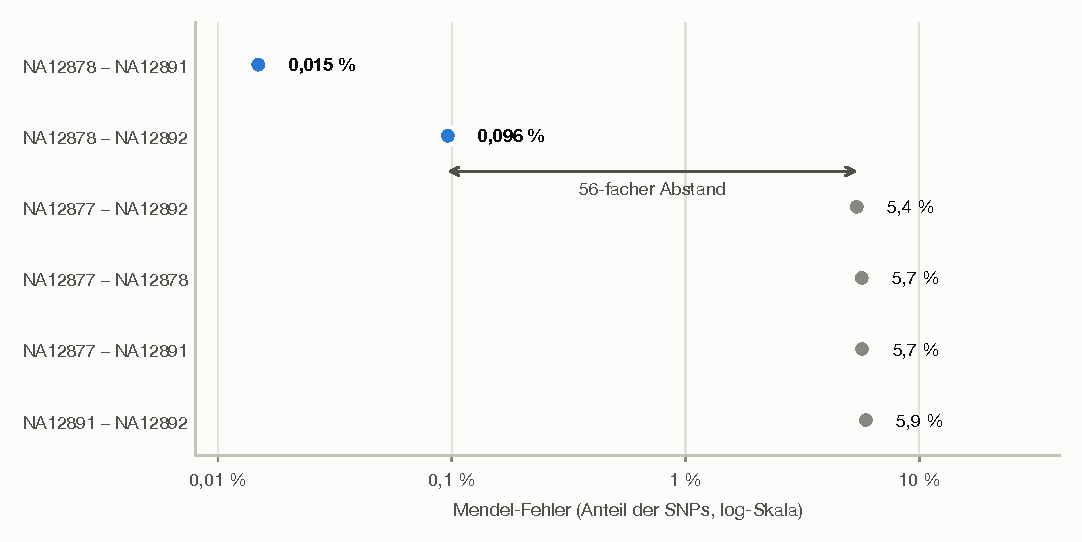
\includegraphics[width=\columnwidth]{abb2_mendel_paare.pdf}
\caption{Mendel-Fehlerrate pro Paar (logarithmische Skala). Blau: Eltern--Kind, grau: nicht verwandt.}
\label{fig:paare}
\end{figure}

\subsection{Trios}
Von den zwölf möglichen Trios hat nur eines eine niedrige Fehlerrate: NA12891 und NA12892 als Eltern von NA12878 mit 2.154 Fehlern (0,654~\%). Die nächstbeste Kombination liegt bei 14,1~\%, also etwa beim 21-Fachen (Abb.~\ref{fig:trioking}a). Damit ist festgelegt, dass NA12878 das Kind ist.

\subsection{Abgeleitete Verwandtschaft}
Abbildung~\ref{fig:netz} fasst beide Ergebnisse zusammen: NA12878 ist das Kind von NA12891 und NA12892, und NA12877 ist mit keiner der drei anderen Personen verwandt.

\begin{figure}[t]
\centering
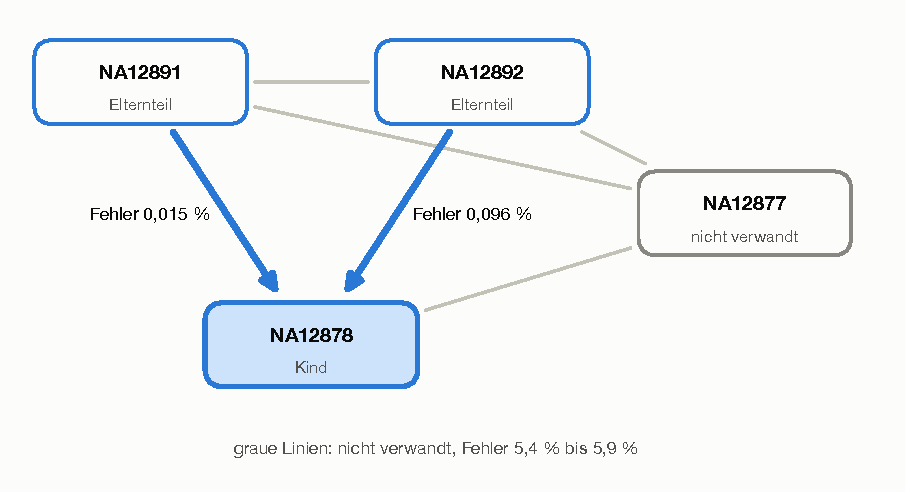
\includegraphics[width=\columnwidth]{abb1_verwandtschaftsnetz.pdf}
\caption{Aus den Genotypen abgeleitete Verwandtschaft. Die Pfeile zeigen von den Eltern zum Kind, die Zahlen sind die Mendel-Fehlerraten der Paare.}
\label{fig:netz}
\end{figure}

\subsection{KING}
KING bestätigt das Bild (Abb.~\ref{fig:trioking}b). Die beiden Eltern-Kind-Paare haben ein IBS0 von 0,00016 und 0,0010, alle anderen Paare liegen zwischen 0,058 und 0,064. Der KINSHIP-Wert liegt für Eltern--Kind bei etwa 0,31 und für die übrigen Paare bei 0,12 bis 0,14, also bei allen Paaren über dem theoretischen Wert.

\begin{figure*}[t]
\centering
\begin{subfigure}[t]{0.52\textwidth}
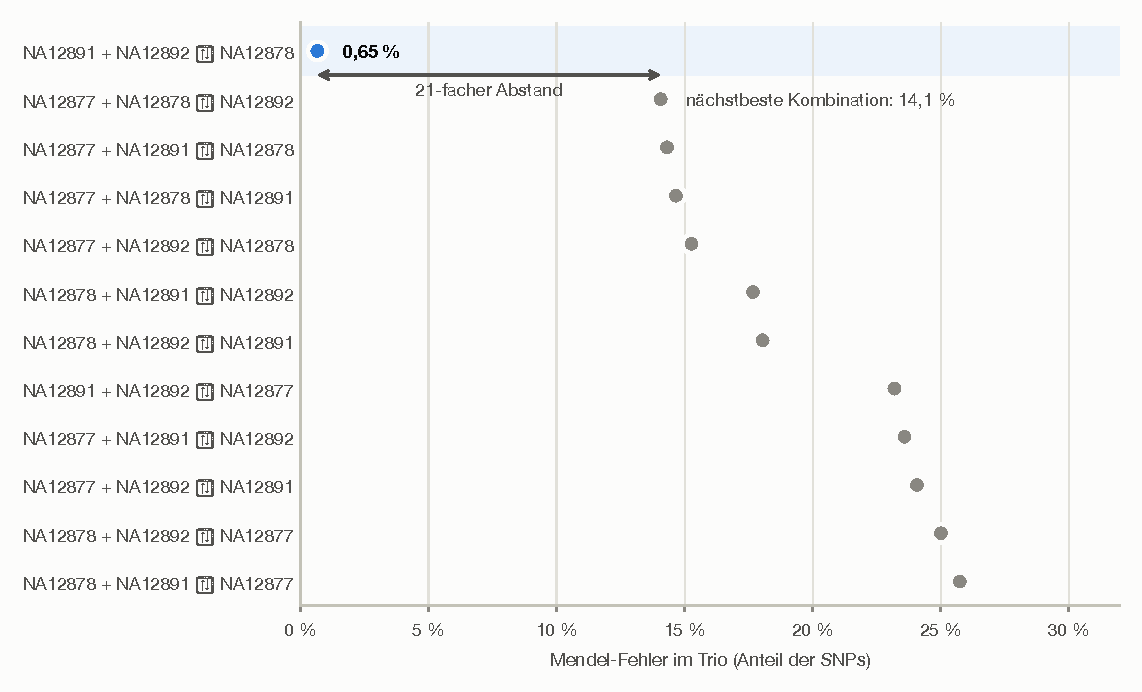
\includegraphics[width=\textwidth]{abb3_mendel_trios.pdf}
\caption{Mendel-Fehlerrate aller zwölf Trios}
\end{subfigure}\hfill
\begin{subfigure}[t]{0.44\textwidth}
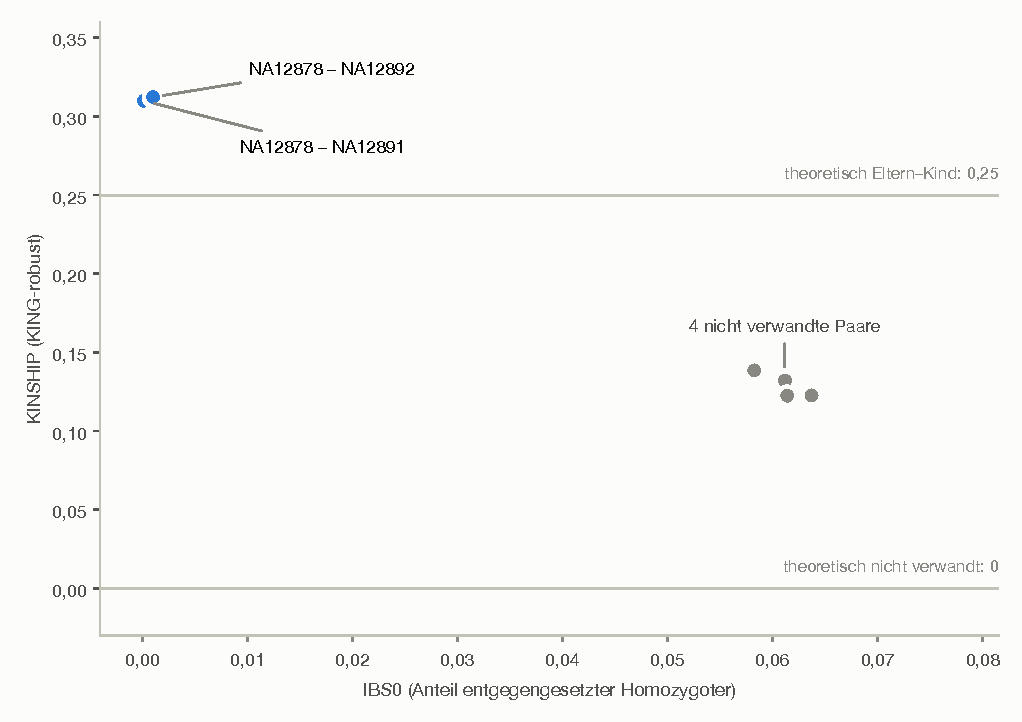
\includegraphics[width=\textwidth]{abb4_king.pdf}
\caption{KING: IBS0 gegen KINSHIP}
\end{subfigure}
\caption{Trio-Auswertung und KING. (a) Das beste Trio ist blau hervorgehoben. (b) Die waagerechten Linien markieren die theoretischen Erwartungswerte für Eltern--Kind (0,25) und nicht verwandt (0).}
\label{fig:trioking}
\end{figure*}

\section{Diskussion}
Beide Verfahren trennen die Paare eindeutig, und die Rangfolge stimmt überein. Das Ergebnis passt zum bekannten Stammbaum der Familie 1463 \citep{eberle2017}: NA12877 ist dort der Partner von NA12878 und damit nicht mit deren Eltern NA12891 und NA12892 verwandt.

Die absoluten KINSHIP-Werte liegen für alle Paare über dem theoretischen Wert (0,31 statt 0,25 bei Eltern--Kind, 0,12 bis 0,14 statt 0 bei nicht verwandten Paaren). Ich vermute, dass die kleine Kohorte aus vier Personen die Allelfrequenz-Schätzung verzerrt, habe das aber nicht überprüft. Belastbar sind deshalb IBS0 und die Rangfolge, nicht die absoluten Werte.

Die Fehlerrate der Eltern-Kind-Paare liegt bei 0,015~\% bis 0,096~\% und nicht bei null. Mögliche Ursachen sind Genotypisierungsfehler, Fehlalignments und seltene \emph{de-novo}-Varianten; eine Aufschlüsselung habe ich nicht vorgenommen.

\section{Einschränkungen}
\begin{itemize}
\item Es wurden nur drei Chromosomen und vier Personen untersucht; die Aussage gilt für diese Daten und ist keine Abstammungsbegutachtung.
\item Mit autosomalen Daten lassen sich Vater und Mutter nicht unterscheiden. Welche der beiden Eltern männlich ist, ließe sich mit Chromosom~X klären.
\item Die Filterschwellen der Genotypen sind nicht an einem Referenzdatensatz kalibriert.
\item Die Ursache der verschobenen KINSHIP-Werte ist nicht geklärt.
\item Die Ergebnisse wurden nur gegen den bekannten Stammbaum eingeordnet, nicht gegen ein unabhängiges Truth Set validiert.
\end{itemize}

\section{Ausblick}
Als nächste Schritte sind die Auswertung von Chromosom~X zur Zuordnung von Vater und Mutter, die Ausweitung auf alle Chromosomen sowie eine Prüfung der verschobenen KINSHIP-Werte (etwa mit externen Allelfrequenzen) vorgesehen.

\section{Schlussfolgerung}
Die Pipeline verarbeitet vier Genome reproduzierbar von den Rohdaten bis zu gemeinsamen SNP-Genotypen. Zwei unabhängige Verfahren leiten übereinstimmend ab, dass NA12878 das Kind von NA12891 und NA12892 ist und NA12877 mit keiner dieser Personen verwandt ist, ohne dass Rollen vorgegeben wurden.

\section*{Datenverfügbarkeit}
Die Sequenzdaten sind öffentlich verfügbar (ENA: ERR194160, ERR194161; NA12877 und NA12878 über die Platinum Genomes). Code und Konfiguration (Snakefile, \texttt{config.yaml}, Skripte) liegen im Projektverzeichnis.

\section*{Anhang: Reproduktion}
Im Projektordner mit aktivierter conda-Umgebung \texttt{trio\_test}:
\begin{lstlisting}[language=bash]
mkdir -p data work
caffeinate -i snakemake -j 8 \
  --resources mem_gb=16 \
  --rerun-triggers mtime
python scripts/plot_results.py
latexmk -pdf bericht.tex
\end{lstlisting}
Der Ordner \texttt{work/} muss existieren, weil Snakemake leere Ordner nach dem Löschen temporärer Dateien entfernt und die Regel \texttt{king} sonst mit \texttt{Failed to open work/cohort.log} abbricht. Software: Snakemake 9.27.0, bwa 0.7.19, samtools 1.24, GATK 4.6.2.0, bcftools 1.24, PLINK 2.0.0a.7.8 und Python 3.11.17 mit Matplotlib 3.11.2.

\bibliographystyle{plainnat}
\bibliography{literatur}
\end{document}
